\begin{figure}[H]
\centering

\includegraphics[scale=0.25]{images/img-004-009.png}
\end{figure}

% Multiple Choice Question 1
\begin{questions}\setcounter{question}{0}\question
A long, cylindrical conductor with inner radius $a$ and outer radius $b$ carries a current $I$ distributed uniformly over its cross section (the shaded region shown above). Which of the following graphs best shows the magnitude of the magnetic field $B$ as a function of the distance $r$ from the axis of the conductor?

\begin{oneparchoices}
\choice \adjustbox{valign=t}{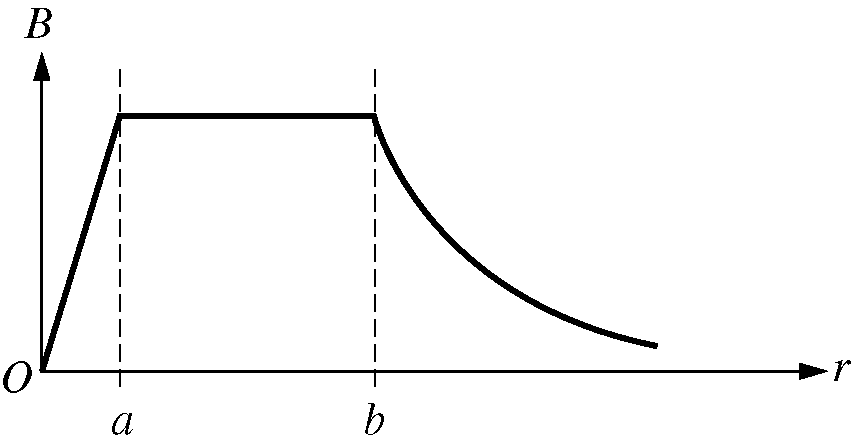
\includegraphics[scale=0.23]{images/img-004-010.png}}
\choice \adjustbox{valign=t}{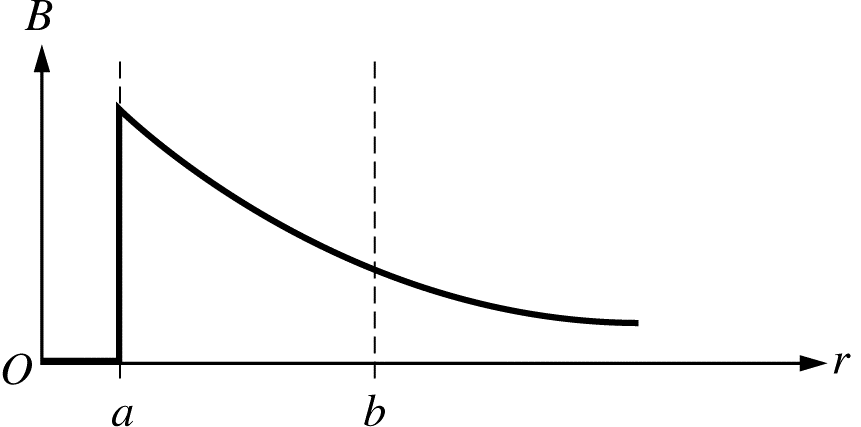
\includegraphics[scale=0.23]{images/img-004-011.png}}
\choice \adjustbox{valign=t}{
\includegraphics[scale=0.23]{images/img-004-012.png}}
\choice \adjustbox{valign=t}{
\includegraphics[scale=0.23]{images/img-004-013.png}}
\choice \adjustbox{valign=t}{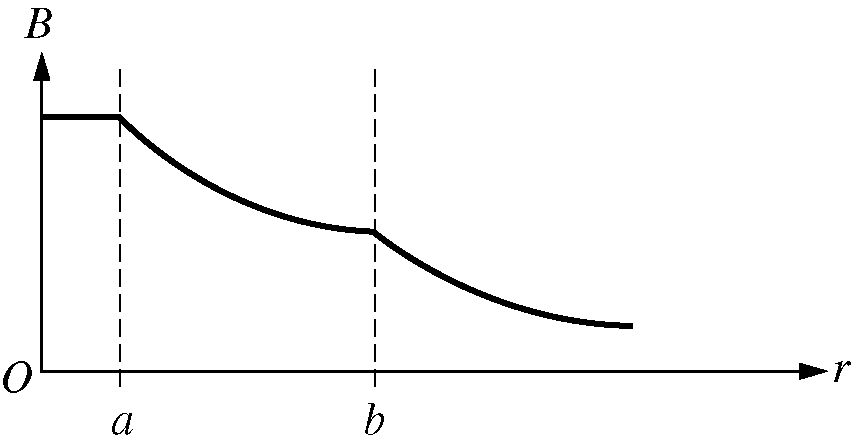
\includegraphics[scale=0.23]{images/img-004-014.png}}
\end{oneparchoices}\end{questions}

